\documentclass[MIRU,submit,english]{miru2019e}
\usepackage{graphicx}
\usepackage{mathtools}
%\usepackage{latexsym}
%\usepackage[fleqn]{amsmath}
%\usepackage[psamsfonts]{amssymb}

\begin{document}

\title{Dog-centric Activity Estimation}

\affiliate{Tokyo}{Department of Informatics, The University of Electro-Communications} %{電気通信大学 大学院情報理工学研究科 情報学専攻}
\affiliate{Tohoku}{NICHe, Tohoku University}
\affiliate{riken}{Organic Physical Chemistry Laboratory} %{理研AIP}

 \author{Tsuyohito ARAKI}{Tokyo}[araki-t@mm.inf.uec.ac.jp]
 \author{Yuta IDE}{Tokyo}%[ide-y@mm.inf.uec.ac.jp]
 \author{Kazunori OHNO}{Tohoku}%[hamada@rm.is.tohoku.ac.jp]
 \author{Kazunori OHNO}{Tohoku, riken}%[]
 \author{Keiji YANAI}{Tokyo}%[yanai@cs.uec.ac.jp]

\maketitle
\section*{Abstract}
%被災地での災害救助を補助する犬をレスキュー(災害救助)犬といい,カメラなどの計測装置を装備したレスキュー犬をサイバーレスキュー犬と言う.
Dogs that assist disaster relief in the affected areas are called rescue dogs, and dogs equipped measuring device such as cameras are called cyber rescue dogs.
%本研究では,犬にとりつけたセンサからサイバーレスキュー犬活動の識別を目的とする.
In this study, we aim to identify the behavior of cyber rescue dog from the sensor attached to the dog.
%犬一人称動画像と音声をCNNを用いて動作毎に分類するsound/image-based three-stream CNNの提案と,提案手法をマルチクラス推定に用いた実験を行なった.
We proposed a Sound/image-based three-stream CNN that classifies dog activity from dog-centric movies and sounds.
And experiment using the proposed method for multiclass estimation.
%Sound/image-based three-stream CNNは動画から得られた静止画像・optical flow画像・音声を入力とする動画識別ネットワークである.
Sound/image-based three-stream CNN is a movie identification network that receives still images, optical flow images, and audio obtained from movie.
%本提案手法の有効性を示すため,3つの入力それぞれ単体とその組み合わせパターン
%(静止画像単体,optical flow画像単体,音声単体,静止画像+optical flow画像,静止画像+音声,optical flow画像+音声)
%を用いた識別との比較実験を行なった.
In comparison experiments to confirm the effectiveness of the proposed method, single pattern and multiple patterns were used for each of the three inputs.
%結果は,51.8\%で提案手法で最も高い精度が得られた.
As a result, the highest accuracy was obtained with the proposed method at 51.8\%.
%推定には,レスキュー犬の訓練の様子を撮影したデータセットを用いた.
For estimation, we used a rescue dog training data set.
%このデータセットは現在も作成中であり,まだ学習のデータ量が十分とは言えない.
This data set is still being created, and the amount of data needed for learning is not enough.
%一人称視点動画からのマルチクラス推定というタスクと,レスキュー犬訓練データセットの複雑さのあいまったチャレンジングなタスクであることを踏まえても不十分な結果であり,今後さらに手法の改良とデータセットの拡充が必要である.
The result is insufficient even if Given the complex dataset of the rescue dog training and the task of multi-class estimation from dog-centric movies.
We need to further refine this method and extend the data set in the future.

\section{Introduction}
%被災地での救助活動を行う際に,人間の補助として訓練されたレスキュー犬(災害救助犬)が探査を行う場合がある.
In rescue activities in the affected areas, trained rescue dogs may conduct surveys as human assistants.
%レスキュー犬は人間とペアを組み,犬としての特性を生かして人間と協力して被災地の探索を行う.
The rescue dog makes a pair with a human and investigate for a affected areas making use of the characteristics as a dog.
%がれきの隙間などの狭い空間や倒壊した建物など人間には踏破困難な環境でも探査可能であり,発達した嗅覚を頼りにした救助活動が可能である.
Resque dogs can investigate even in environments where it is difficult for a person to traverse on such as a narrow space and a crevice or a collapsed building.
And a rescue operation that relies on the developed sense of smell is possible.
%しかし彼らは人間に向けた言語を持たない.
However, they have no language for humans.
%ペアを組む人間はハンドラーと呼ばれ、ハンドラーはレスキュー犬の行動から彼らが収集した情報を理解しなくてはならない.
%People in pairs with rescue dogs are called handler, and handlers must interpret the information that collected by rescue dog from there behavior. %ここよくわかりません by araki.
People in pairs with rescue dogs are called handler, and handlers must interpret from rescue dog's behavior the information that they collected.
%現状では,レスキュー犬を指揮するハンドラーと呼ばれる人間がレスキュー犬の行動を手動でマーキングしており,その情報を消防などの指揮命令者に口頭伝達している.
Under the present circumstances, a handler who directs a rescue dog manually marks the action of the rescue dog and orally transmits information to a commander such as a fire department.
%このレスキュー犬との共同探索の問題点として,トリアージ(緊急度に従った手当の優先順位付け)のための周辺環境情報や,要救助者情報の不足があげられる.
As a problem of joint investigation with this rescue dog, there is a lack of information on surrounding environment and victims for triage.
%また,ハンドラーによる記録はどうしても主観的になるので客観性に欠け,さらにそれが口頭伝達されることで正確性がより欠落する.
And, the records by the handler are subjective, so they lack objectivity. Verbal transmission also makes them less accurate.
%本研究では,レスキュー犬にセンサを装着して得られたデータを用いてレスキュー犬の行動推定を目的とする(Figure\ref{lite_model}).
In this study, we aim to estimate the behavior of rescue dogs using data obtained by attaching sensors to rescue dogs (Figure\ref{lite_model}).
%本研究の具体的なタスクは, 映像だけでなく音声などのデータも活用したマルチモーダル情報を用いたクラス推定である.
The specific task is class estimation using multimodal information that uses not only video but also audio data.
%これにより,レスキュー犬が今何をしているのか個人の主観に基づくことなく判断することが可能となり,
As a result, this makes it possible to determine mechanically what the rescue dog is doing now.
%トリアージに必要な情報が整理され,災害救助活動の効率化が期待される.
And, information necessary for triage is organized, disaster rescue activities will be more efficiently.

\begin{figure}[tb]
 \begin{center}
%  \includegraphics[width=7cm]{./Figures/easy_image.eps}
  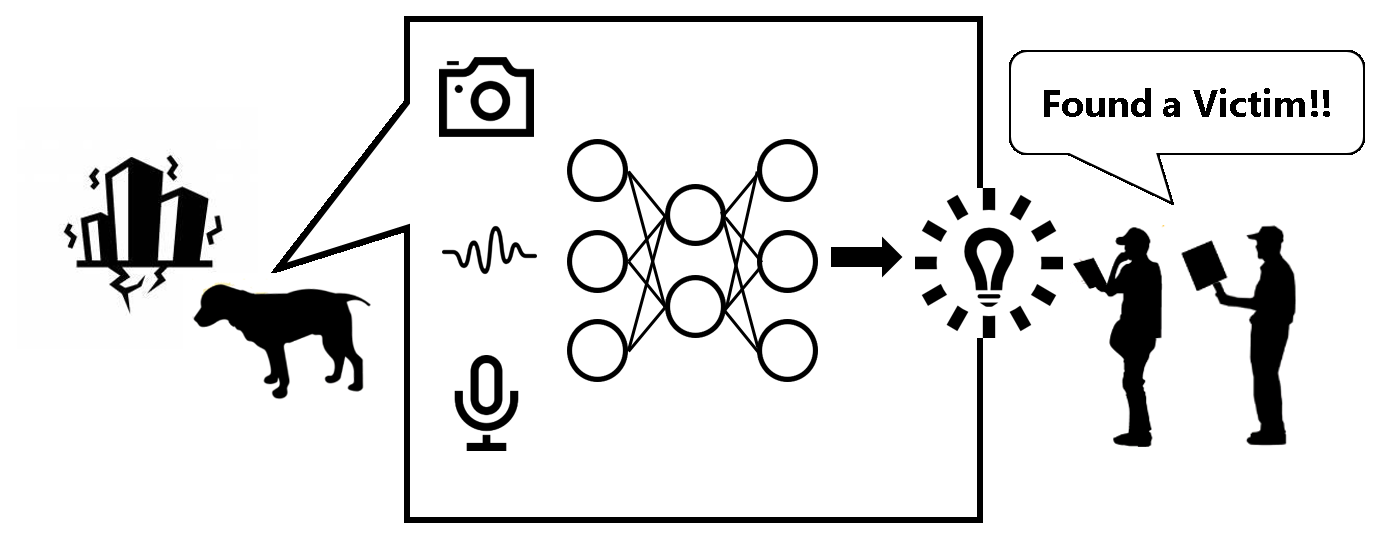
\includegraphics[width=7cm]{./Figures/dogactrec.eps}
  %\caption{提案手法の概要.入力画像から複数データを抽出し,それぞれ別のストリームへ入力する.各ストリームの出力をもとに,動画のレスキュー犬行動推定結果を最終出力とする.}
  \caption{Outline of the proposed method. Extract multiple data from the input image and enter them into different streams. Based on the output of each stream, estimate the rescue dog behavior.}

  \label{lite_model}
 \end{center}
\end{figure}

\section{Related Work}
%動画分類の研究に two-stream CNN ~\cite{simonyan2014two}がある.
There are two-stream CNN as a study of video classification ~\cite{simonyan2014two}.
%これは動画のフレームとフレームから求まる optical flow画像を個別のネットワークで学習することで動き情報を考慮した動画分類を行っている.
It is classify videos by learn motion information from optical flow image that calculated between frame and frame.
%レスキュー犬行動のモニタリングのために,大野, 濱田らによって装着型計測・記録装置が開発された~\cite{dog01}.
Ohno, Shibata et al. Developed a wearable measurement recording device for monitoring of rescue dog behavior ~\cite{dog01}.
%Figure~\ref{cyber}にレスキュー犬に装着可能な軽量な行動計測スーツを示す.
We show that attachable device with rescue dog Figure~\ref{cyber}.
%これを着用したレスキュー犬はサイバー救助犬とも呼ばれる.
Rescue dogs wearing that called cyber rescue dogs.
%各種センサを用いた計測データを記録し,リアルタイムに映像などのデータを無線配信することが可能である.
This device can record measumented data and broadcast information as a movie and so on.
%そのため,レスキュー犬が人の目の及ばない範囲で活動する際にもレスキュー犬の行動やその周辺環境などを把握するのに役立つ.
It makes handler can understand the beyond rescue dog activity that over the rubble.

%また,Ehsanらによる犬の一人称視点動画からの犬行動予測の研究がある~\cite{whoretthedog}.これは,犬の行動をモデリングし,犬が次にどのような道をたどり行動するかを予測している.
Also, there are study that estimated dog activity from dog-centric video by Ehsan. at al.
It is modeling dog activity and estimate how dogs will move.
%しかし,これらの研究は犬の行動のモデリングであり,犬の周辺環境の推定などは行っていない.
%また,入力は動画像のみであり,音声などのデータは利用していない.
However, that study used only video, not used multimodal information such as audio.
%レスキュー犬の課題には,犬の周辺環境情報や動画像からだけでは判断できない情報の取得が含まれている.
Rescue dogs are asked more information that can be judged not only from the dog's surrounding environment information and moving images.
%例えばレスキュー犬は要救助者を発見するとその場で待機し吠え続けるように訓練されている.
For example, rescue dogs are trained to stay on the spot and continue to bark when they find a victim.
%このように,動画像データからだけではなく,音声データ,および慣性データ・GPSデータなどの情報を複合的に用いてレスキュー犬の状態を判断しなければならない.
In this way, handler must understand the surrounding environment of the rescue dog using not only video data but also information such as voice data, inertia data and GPS data in combination.
%ただし, 本研究では動画像と音声情報のみの提供をうけたため, これらを入力とした犬の行動推定を行う.
But, we has been provided only dog-centric motion pictures and voice information, in this study use these inputs for estimate the activity of rescue dogs.

%音声に焦点をあてた動画分類の研究にはSoundNet~\cite{aytar2016soundnet}がある.
SoundNet as a study of movie classification focus it's sounds ~\cite{aytar2016soundnet}.
%動画から音声と画像を取り出し,画像を教師データとし,音声は生徒データとして出力が等しくなるように学習している.
In the SoundNet, deep convolutional sound network is trained with with visual supervision.
%この手法は音響シーン分類,物体分類の標準ベンチマークにおいて教師あり学習の最高精度を達成した.
This method achieved the state-of-the-art results on standard benchmarks for acoustic scene/object classification. 
%本研究では音声のみからの行動推定は目的としない.しかし,音声の意味的情報は動画認識に重要であることが明らかにされている.
Semantic information of audio has been shown to be important for movie recognition, we don't aimed classification from only audio. 
%SoundNetとtwo-stream CNN を参考に, 本研究では音声識別ネットワークと two-streamネットワークを統合したアーキテクチャを構築した.
In this study build the architecture connected two-stream network with deep audio network while refering to SountNet and two-stream CNN.
%SoundNetが音声波形を入力とするのに対し,本研究では音声からMFCC特徴を抽出してからストリームへの入力とする点で異なっている.
SoundNet takes an audio waveform as an input. 
On the other hand, this study is different in that it extracts MFCC features from audio and then uses them as input to a stream.

%音声と動画像だけでなく,加速度と速度情報を用いたマルチモーダルな学習の研究には丹野らの~\cite{tanno2019deim}がある.
There is research of multimodal learning using not only audio and moving pictures but also acceleration and speed information by Tanno et al ~\cite{tannno2019deim}.
%これは,情報を追加することによっての認識精度の向上や低下を報告しており,特に音声によって分類精度が向上するとされている.
That research reported that improvement and decrease in recognition accuracy by adding information.
In particularly, classification accuracy is improved by audio. 
%マルチモーダルな深層学習という点で本研究と同様のテーマだが,マルチクラス推定という点で本研究とは異なっている.
It is the same theme as this study in terms of multimodal deep learning, but it differs from this study in terms of multiclass estimation.

\begin{figure}[tb]
 \begin{center}
  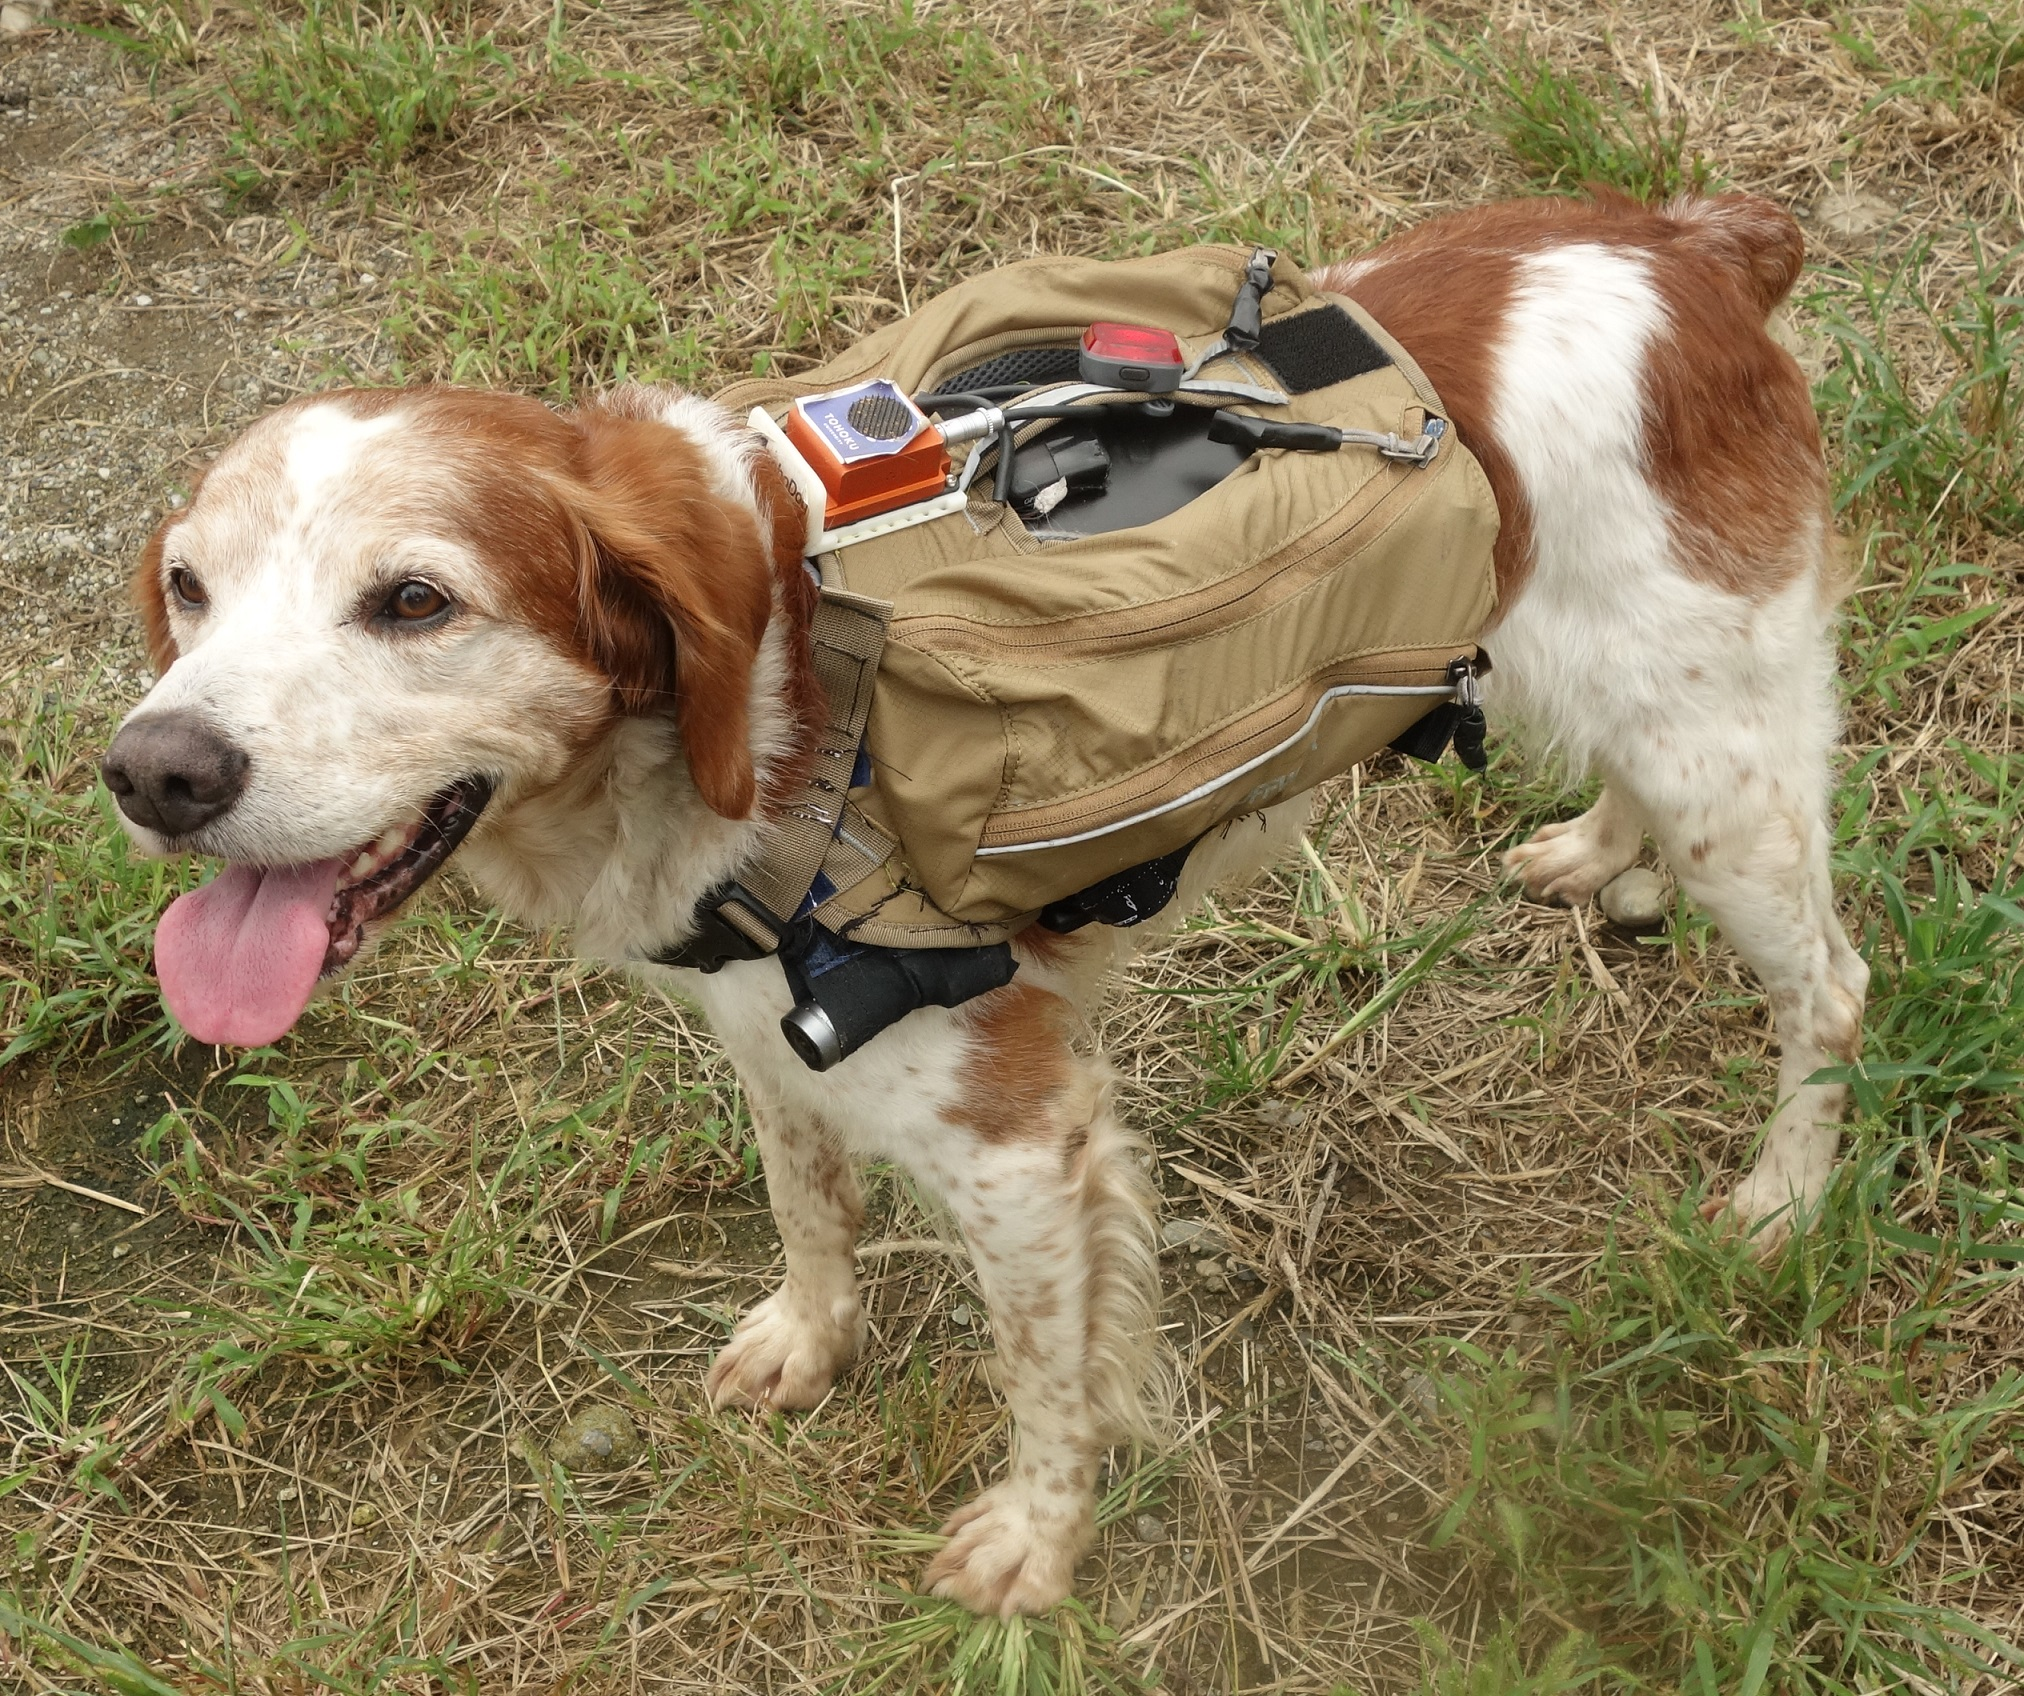
\includegraphics[width=5cm]{./Figures/cyberdog.eps}
  %\caption{装着型計測・記録装置~\cite{dog01}より引用.}
  \caption{Wearable measurement and recording device ~\cite{dog01}.}
  \label{cyber}
 \end{center}
\end{figure}

\section{Dateset}
%学習には,サイバーレスキュー犬訓練データセットを利用した.
We use the Training Cyber Rescue Dog Dataset.
%これは,訓練されているレスキュー犬に専用の計測スーツを着用させ収集したデータ群である.東北大学の大野らからその一部を提供された.
This is data collection about training rescue dog wearing recoding device. We are provided some piece of that datas by Ohno et al.
%提供されたデータは7本からなる動画で, 時間の範囲を指定するように犬行動がラベル付けされている.
Provided data consists of seven movies, each movie has three view point: dog-centric, handler-centric and third-person view.
Each view are labeled rescue dog activities based on time lange.
%犬行動は11種(bark:吠える, cling:匂いに執着する, command:ハンドラーからの働きかけがある, eat-drink:飲食する, look\_at\_handler:ハンドラーを見る, run:走る, see\_victim:要救助者を発見した, shake:体をブルブルと震わせる, sniff:匂いを嗅ぐ, stop:脚を止める, walk-trot:歩く)あり, その一部をFigure~\ref{dataset}に示す.
There are 11 classes of rescue dog activities: bark, cling\_to\_something, command\_by\_handler, eat-drink, look\_at\_handler, run, see\_victim, shake\_body, sniff, stop\_legs and walk-trot.
Figure ~\ref{dataset} show part of that.
%分類クラスそれぞれについて時間範囲を指定する形で動画にアノテーションがされており,同時刻に複数のクラスが重なるためマルチラベルデータとして取り扱う.
Each class annotated every movies to specifying time lange. Because multiple classes overlap at the same time, it is treated as multi-label data.

%総時間は57分40秒,秒間フレーム数は29.97,総フレーム数は103,696枚である.
Total time is 57 minutes and 40 seconds, 29.97 FPS, the number of frames is 103,696.
%これを 6fpsにサンプリングして整形したものを学習と評価に用いた.
We thinned the frames to 6fps for use to train and evaluation. 
%クラス毎の出現頻度が~表\ref{cyberdataset_label}の値である.表記のためクラス名を簡略した.
Table ~\ref{cyberdataset_label} shows the frequency of occurrence of each class. Class names are abbreviated for convenience of notation.
%各クラス毎に約100回から9000回のサンプルがあり数値上では十分である.
Each class has 100 to 9,000 samples, so it looks numerically good enough.
%しかしこれは連続したシーンを含めての数値であり,その実は多様性に欠ける中身となっている.
However, there are continuous scenes. Therefore, the content of the data is actually lacking in diversity.
%例えば,runクラスは98サンプルあるが,独立したシーンとしては3シーンにすぎず,
For example, the class `` run '' has 98 samples, but only 3 scenes as independent scenes.
%bark,eat-drink,see\_victim,shakeクラスを合わせても100シーンに満たない.
Also, the sum of scene ``bark'', ``eat-drink'', ``see\_victim'' and ``shake\_body'' is less than 100 scenes.

\begin{table*}[htb]
 \begin{center}
 %\caption{サイバーレスキュー犬訓練データセット 利用範囲内で計測した出現回数}\label{cyberdataset_label}
 \caption{Class frequency of occurrence of Training Cyber Rescue Dataset}\label{cyberdataset_label}
 \scalebox{0.95}[0.95]{
  \begin{tabular}{|l||c|c|c|c|c|c|c|c|c|c|c|}
   \hline \hline
      Class name   & \rotatebox{90}{bark}& \rotatebox{90}{cling}&\rotatebox{90}{command}& \rotatebox{90}{eat}&\rotatebox{90}{handler}& \rotatebox{90}{run}&\rotatebox{90}{victim}& \rotatebox{90}{shake}& \rotatebox{90}{sniff}& \rotatebox{90}{stop}& \rotatebox{90}{walk} \\ \hline

%   ラベル & bark&cling&comm&eat&handler&run&victim&shake&sniff&stop&walk \\ \hline
   Occurrence& 1744& 1127&2439&343&  2011& 98&  1549&  239& 7719&6384&8764 \\ \hline
  \end{tabular}
 }
\end{center}
\end{table*}

%フレームの静止画像とその直後のフレームから計算したoptical flow画像, および前後15フレーム分の長さの音声の3データをフレーム毎に抽出した.
Three data were extracted for each frame: still image, optical flow image calculated from immediately frame and 15 frames of audio before and after the frame.

\begin{figure}[tb]
    \begin{tabular}{l}

      \begin{minipage}{0.32\hsize}
        \begin{center}
          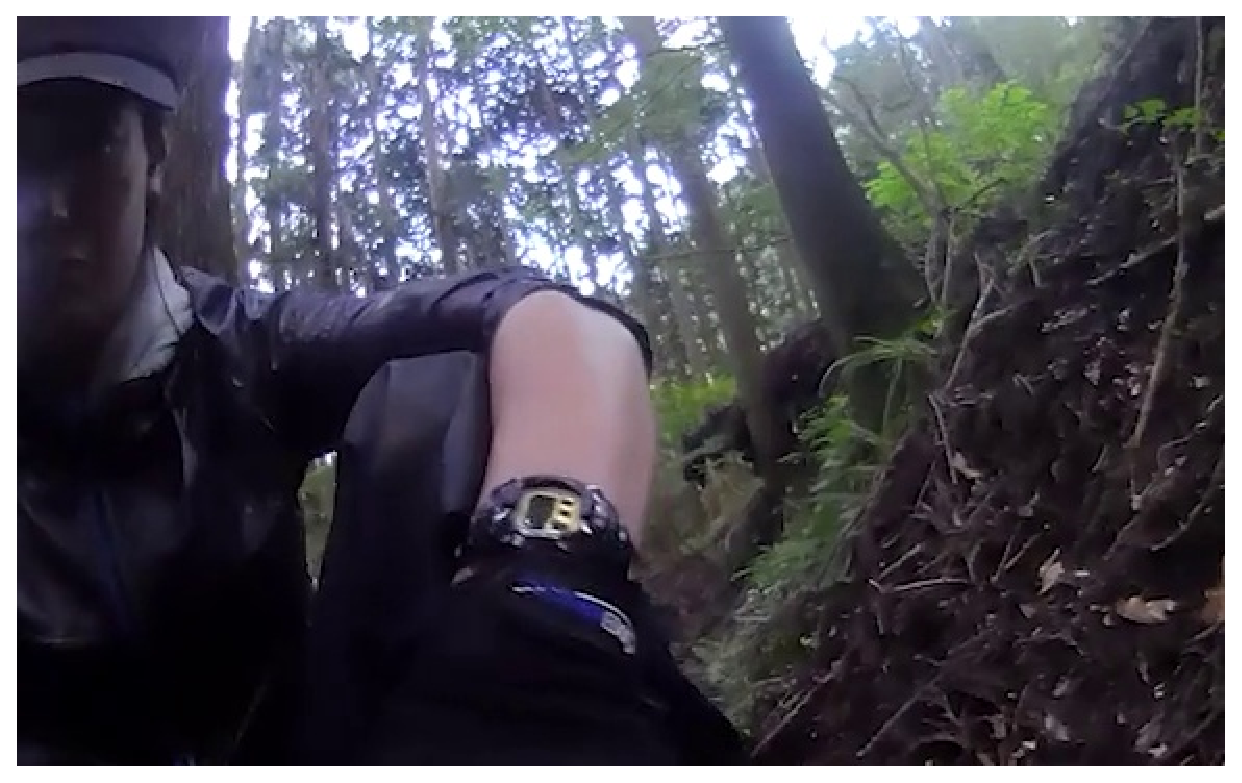
\includegraphics[clip, width=2.8cm]{./Figures/still_seevictim3.eps}
        \end{center}
      \end{minipage}

      \begin{minipage}{0.32\hsize}
        \begin{center}
          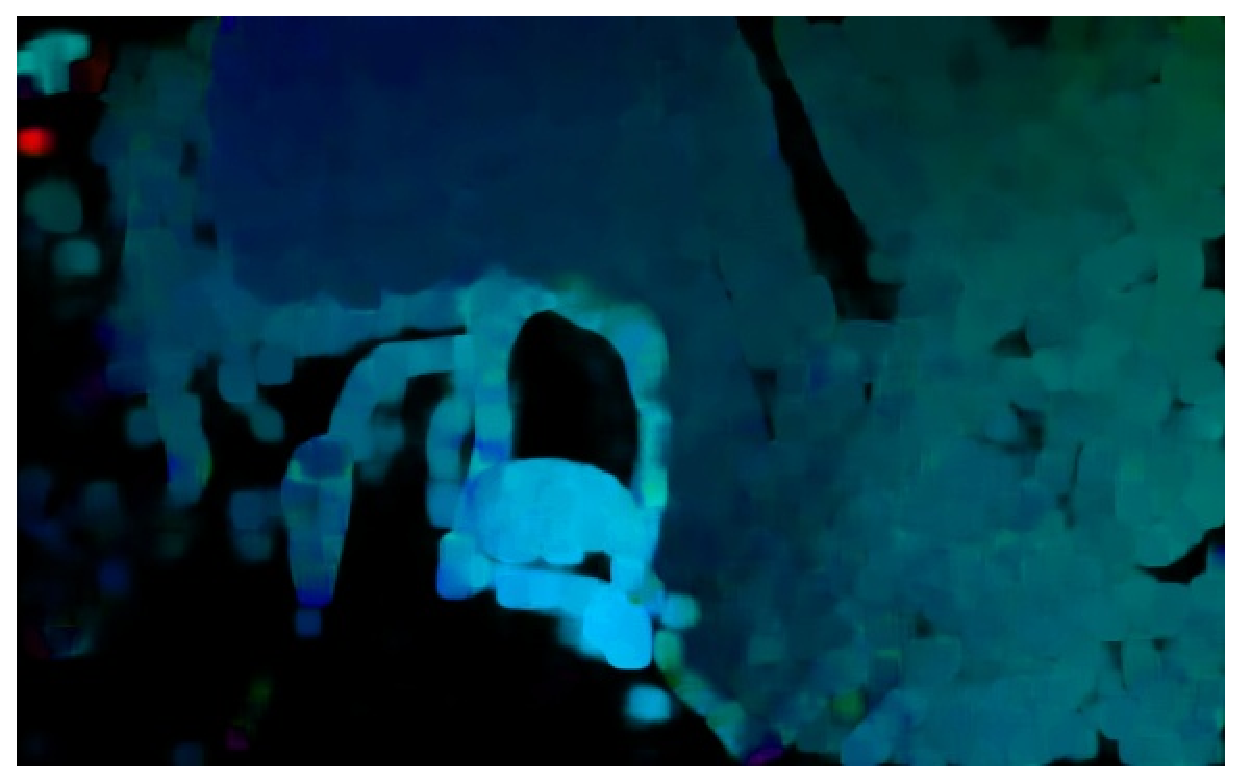
\includegraphics[clip, width=2.8cm]{./Figures/optic_seevictim3.eps}
           %\hspace{2.0cm} {}
        \end{center}
      \end{minipage}

      \begin{minipage}{0.32\hsize}
        \begin{center}
          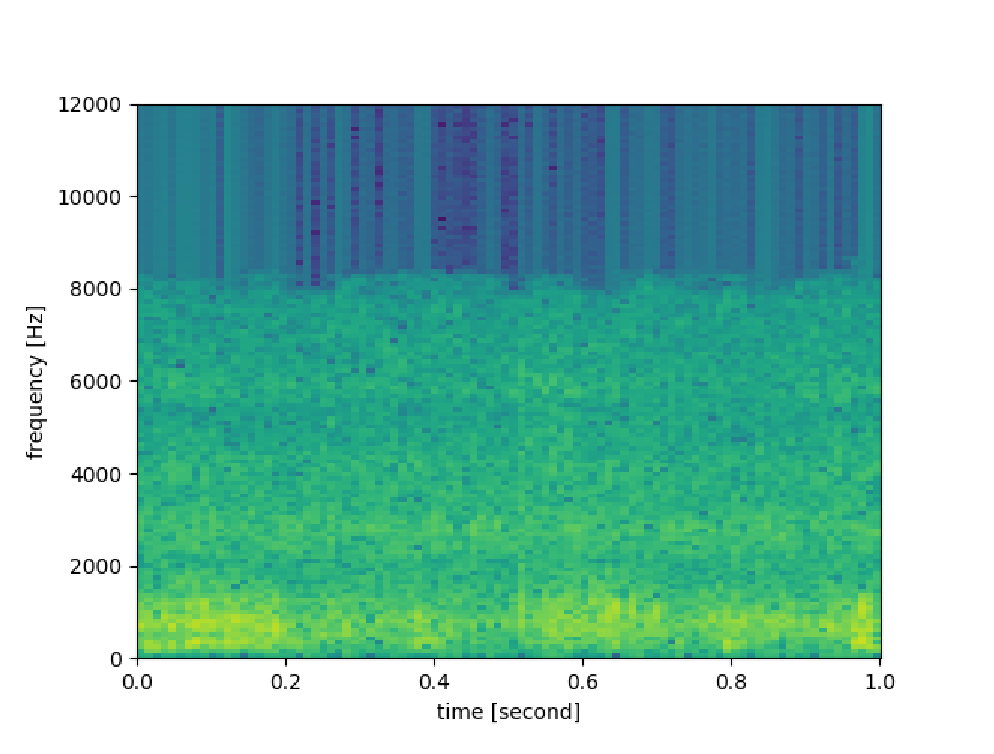
\includegraphics[clip, width=2.8cm]{./Figures/sound_seevictim.eps}
        \end{center}
      \end{minipage}
%    \end{tabular}
\\  %%%%%%%%%%%%%%%%
      \begin{minipage}{0.32\hsize}
        \begin{center}
          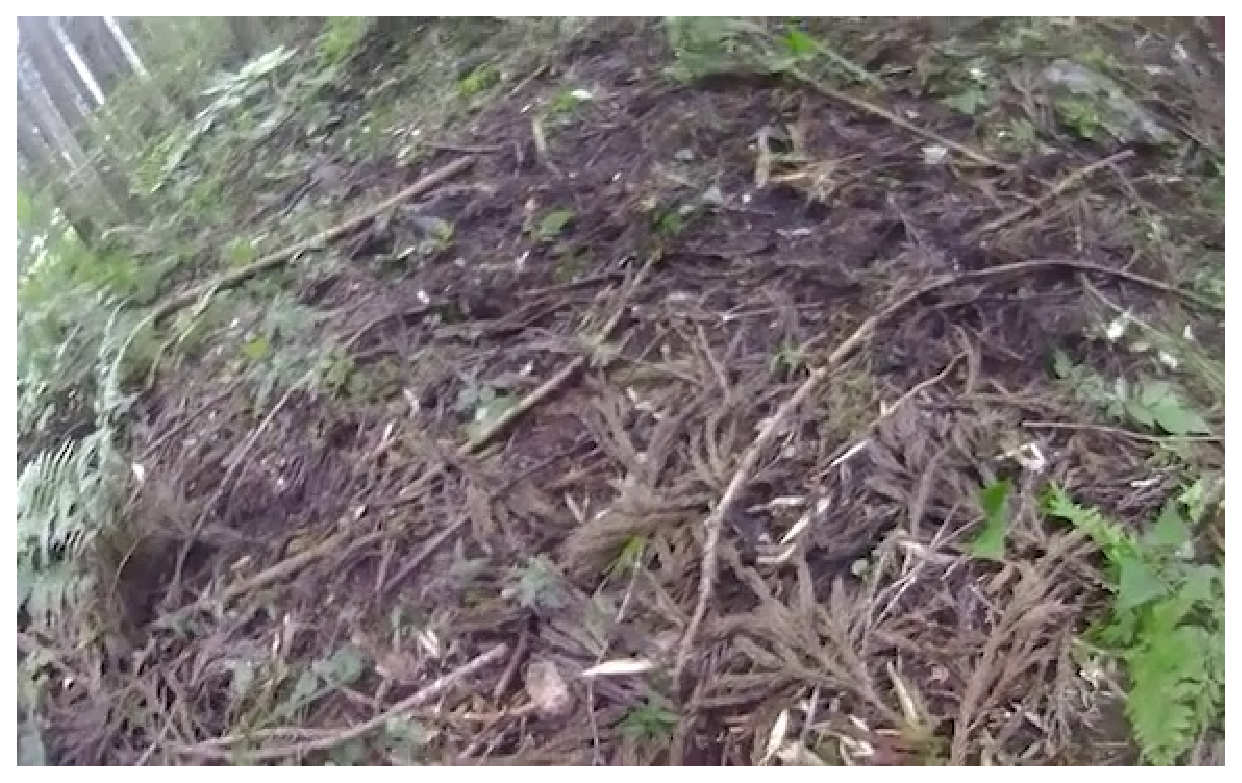
\includegraphics[clip, width=2.8cm]{./Figures/still_stop1-3.eps}
        \end{center}
      \end{minipage}
      \begin{minipage}{0.32\hsize}
        \begin{center}
          
\includegraphics[clip, width=2.8cm]{./Figures/optic_stop1-3.eps}
        \end{center}
      \end{minipage}
      \begin{minipage}{0.32\hsize}
        \begin{center}
          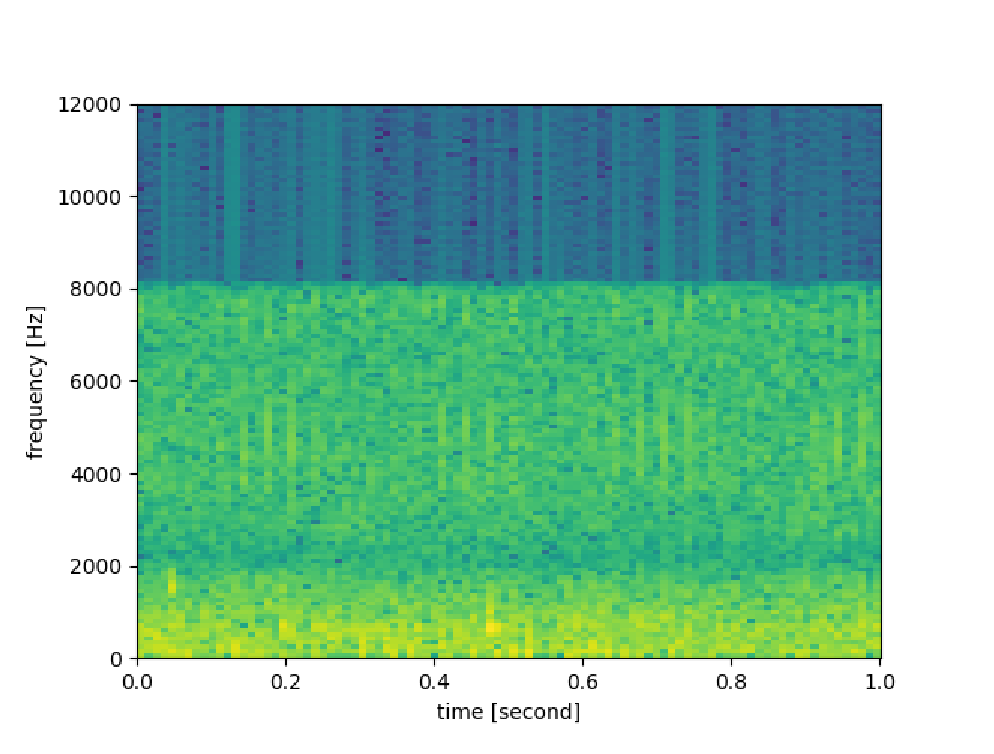
\includegraphics[clip, width=2.8cm]{./Figures/sound_stop2.eps}
        \end{center}
      \end{minipage}
    \end{tabular}
    %\caption{サイバーレスキュー犬訓練データセットsee victimクラス(上段)とstopクラス(下段). 左から静止画像, optical flow画像, MFCCスペクトラムで可視化した音声である.}
    \caption{Class ``see victim'' (upper) and class ``stop'' (lowwer) from Training Cyber Rescue Dataset. From the left, still image, optical flow image and audio data visualized by MFCC spectrum.}
    \label{dataset}
\end{figure}


\section{Proposed Method}
本研究ではレスキュー犬の行動推定のために,動画像・音声のマルチラベル推定を行う.
そのため,レスキュー犬訓練データセットを認識するためのsound/image-based three-stream CNNを提案する.
これは,two-stream CNN に音声ストリームを加えたモデルである.静止画像, optical flow画像, 音声を別々のストリームへの入力とし,それぞれの出力を元にレスキュー犬の行動を推定する.
Sound/image-based three-stream CNN のアーキテクチャをFigure~\ref{sound3st}に示す.

まず入力となる動画から静止画像のフレーム($F_t$)を取り出し,直後の$F_{t+1}$間とのoptical flow画像($O_t$)を生成する.次に両画像から同じ構造の2つのネットワークを用いて特徴量の抽出を行う.
そして対応する音声($A_t$)からMFCC($M_t$)を求め,前述とは異なる構造のネットワークを用いて($M_t$)から特徴量の抽出を行う.
最後にこれら2つあるいは3つの特徴量の組み合わせ毎に結合し,分類ネットワークでクラス分類を行う.
この際に,音声をフレームと同じサイズで切り出すと特徴が著しく失われるため入力音声には$F_t$の前後0.5秒ずつを用いた.動画あるいは音声から実際に犬の行動を推定する場合を想定し,現実的で取り扱いやすい時間としてこれを設定した.
動画長は31フレームとし,中央から切り出した静止画像とそれに対応する直後のoptical flow画像をそれぞれImageNetで学習済みのVGG16モデルに通し,畳み込み層の出力を結合した.
動画から切り出した音声は畳み込みを繰り返すと特徴の縦横次元が小さくなるため,静止画像の畳み込みの出力と同じサイズになるように調整した.
調整は畳み込みで奥行き次元を揃えた後,同じ特徴をリピートし目的の大きさになるまでコピーして結合した.
分類はフレーム毎に行った.
推定にはクラス毎にSoftMarginLossを用いた.
入力を$x$,出力を$y$,クラス数を$C$とすると,マルチクラス推定の損失関数SoftMarginLossは式~\ref{softmargin}に定義される.
推定クラスが正解なら$\Sigma$内の第2項,不正解なら第1項が計算に利用するように設計されており,推定ラベルによって関数が変わる.
本研究では11クラスを取り扱うため,出力yは11次元のバイナリとする.
閾値=0.5とし,閾値以上のクラスを推定クラスとした.
\begin{equation}
    \label{softmargin}
    \begin{split}
    loss(x, y) = &-\frac{1}{C} * \Sigma_{i} y[i] * log((1+exp(-x[i]))^{-1}])\\
    &+ (1 - y[i]) * log(\frac{exp(-x[i])}{1+exp(-x[i])})
    \end{split}
\end{equation}

学習は全てにおいて100エポック行った.学習率は1e-03〜1e-06,バッチサイズは32〜128の範囲で学習毎に変え制限の中で最も良い精度の結果を評価した.

\begin{figure}[tb]
   \begin{center}
    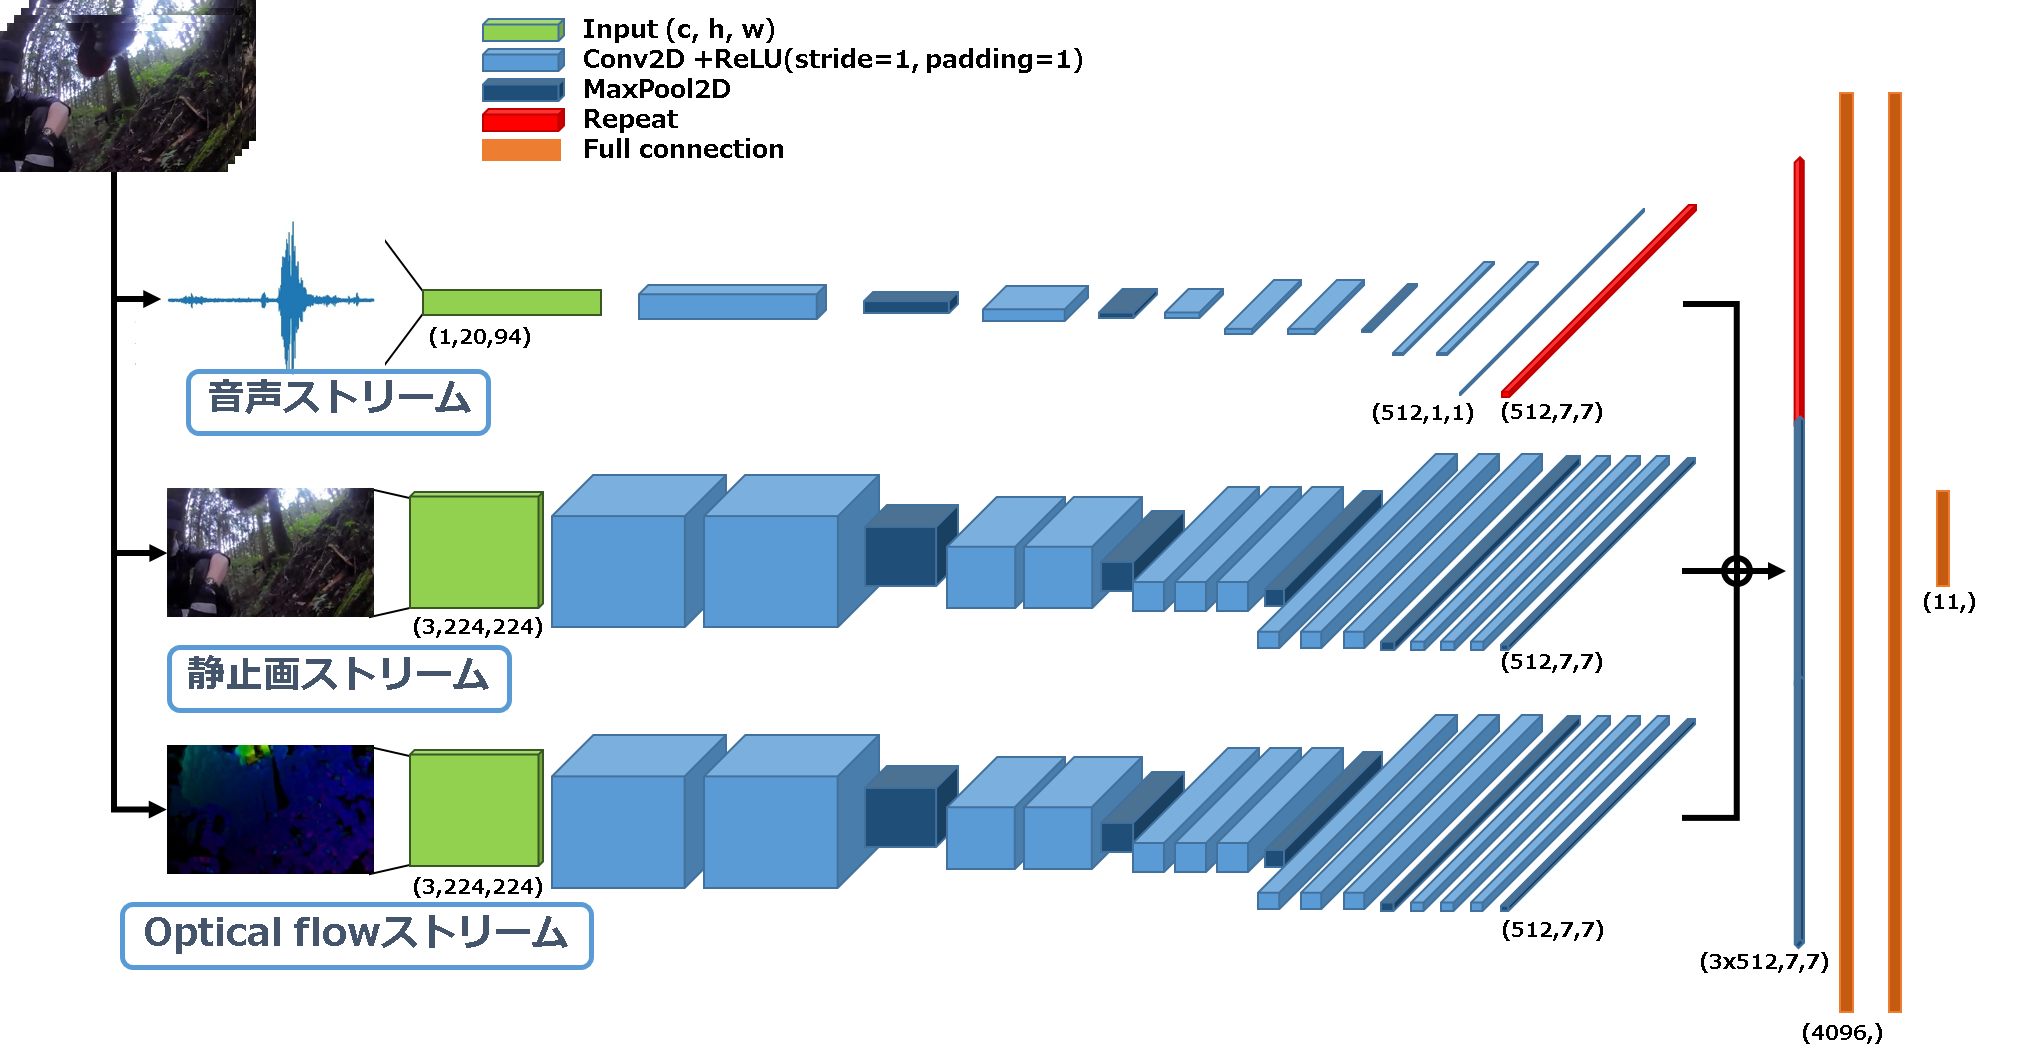
\includegraphics[scale=0.25]{./Figures/soundimage-basedthree-streamCNN.eps}
    \caption{Sound/image-based three-streamアーキテクチャ.音声, 静止画像, optical flow画像それぞれを入力とする3ストリームからなり, それぞれの出力を結合してクラスを推定している.}
    \label{sound3st}
   \end{center}
\end{figure}

\section{Experiments}

3つの入力について, それぞれ単体, 2つずつの組み合わせおよび全てを統合した場合の8通りを行った.%(表~\ref{ablation}).
画像単体を入力とした実験ではImageNetを学習したVGG16の学習済みモデルを用い再学習した.
音声での学習は畳み込み層について1Dと2Dの2種類で行った.
畳み込み層の次元の差についてFigure~\ref{1d2dconv}に詳細を示す.出力の向きを合わせるために, 提案手法の複数入力には2Dの畳み込みを用いた.
一人称視点動画像からのマルチ行動推定を行なった先行研究は見つけられなかったため,既存手法との比較は行なっていない.
表では,クラス毎の精度と全体を合計しての精度をJaccard係数で示している.
なお,Jaccard係数とは$$\frac{TP}{FP+FN+TP}$$で表され,PrecisionとRecallの両者についてF尺度と比較してより厳格な値が求まる.
レスキュー犬の行動分類にあたり,PrecisionとRecallを共に重視するためにこの係数を採用した.
よって,本研究ではJaccard係数がより大きいモデルは精度がより良いと表現する.

結果のまとめを表~\ref{expetiments_result}に示す.
静止画像, optical flow画像単体では精度が低く, これらを組合せたもので精度が上昇した.
比較して, 音声単体では1D, 2Dともに精度が高かった.音声と静止画像,音声とoptical flow画像を組合せた実験では,音声単体と比較して全体的な精度は低下した.
しかし,静止画像, optical flow画像, 音声の3つを組合せた提案手法では全体的な精度の上昇が見られ, クラス別で見ても半数以上のクラスの数値が上昇している.
人間が耳で聞いた際にもその特徴を識別しやすいbark, shakeクラスにおいては音声単体を1D畳み込み層で学習したものの方が数値が高い.
これらから, データセットに対する提案手法の有効性が示された.

\begin{figure}[tb]
   \begin{center}
    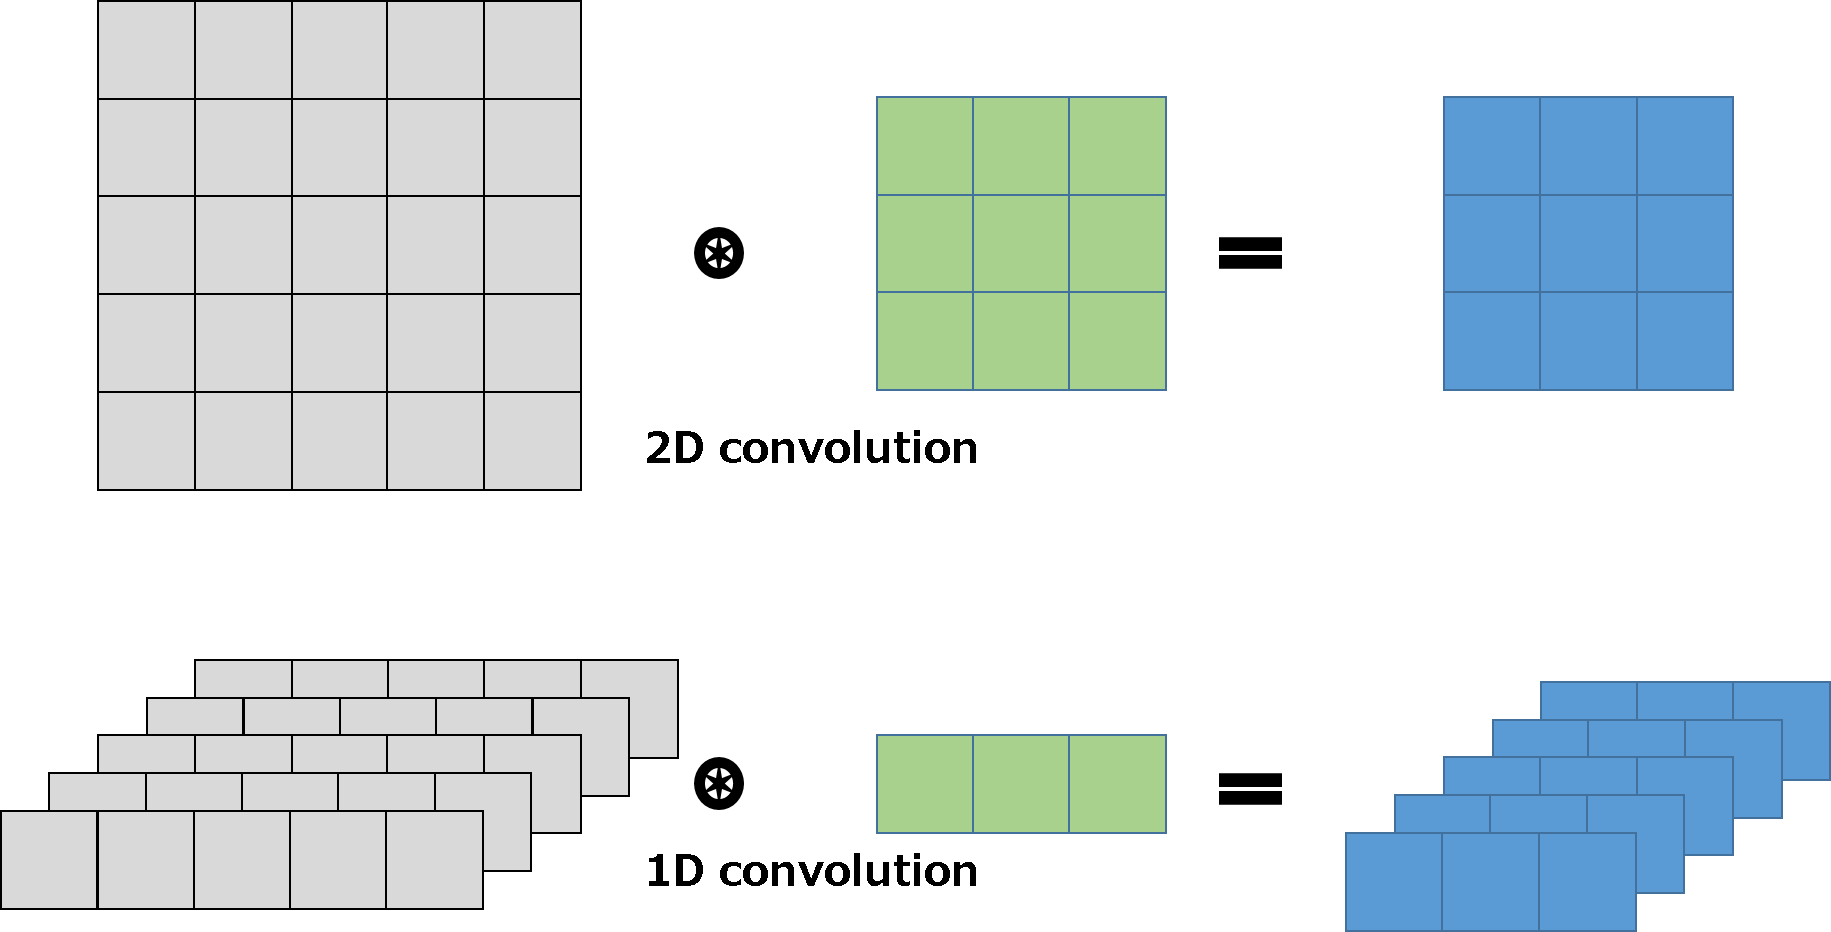
\includegraphics[scale=0.16]{./Figures/1d2dconv.eps}
    \caption{1D convolutionと 2D convolutionの詳細.データは同様でも入力の形と処理が異なり, 出力の結果も異なっている.}
    \label{1d2dconv}
   \end{center}
\end{figure}

\begin{table*}[htb]
% \centering
 \begin{center}
 \caption{各実験結果比較表.}\label{expetiments_result}
 \scalebox{0.85}[0.85]{
  \begin{tabular}{|l|c|c|c||c|c|c|c|c|c|c|c|c|c|c|c|}
   \hline \hline
   &静止画像&optical flow画像&音声& \rotatebox{90}{bark}& \rotatebox{90}{cling}&\rotatebox{90}{command}& \rotatebox{90}{eat}&\rotatebox{90}{handler}& \rotatebox{90}{run}&\rotatebox{90}{victim}& \rotatebox{90}{shake}& \rotatebox{90}{sniff}& \rotatebox{90}{stop}& \rotatebox{90}{walk} & \rotatebox{90}{全体}\\ \hline \hline
(1) & ◯ & × & ×  & 0.244& 0.066& 0.0& 0.024& 0.057& 0.0& 0.204& 0.0& 0.0& 0.588& 0.51&  0.436 \\ \hline
(2) & × & ◯ & ×  & 0.141& 0.0& 0.0& 0.0& 0.017& 0.0& 0.017& 0.0& 0.0& 0.586& 0.476&  0.406 \\ \hline
(3) & × & ×  &1D  & {\bf 0.669}& 0.078& 0.22& 0.023& 0.138& 0.0& 0.274& {\bf 0.44}& 0.502& 0.745& 0.704&  0.512 \\ \hline
(4) & × & ×  &2D  & 0.563& 0.04& 0.188& 0.001& 0.059& 0.0& 0.201& 0.304& 0.524& 0.744& {\bf 0.74}&  0.512 \\ \hline
(5) & ◯ & ◯ & × & 0.11& 0.018& 0.043& 0.0& 0.155& 0.0& 0.259& 0.0& 0.426& 0.705& 0.668&  0.435 \\ \hline
(6) & ◯ & × &2D & 0.662& 0.031& 0.195& 0.018& 0.115& 0.002& 0.308& 0.402& 0.498& 0.726& 0.694&  0.5 \\ \hline
(7) & × & ◯ &2D & 0.667& 0.054& {\bf 0.234}& 0.014& 0.123& 0.01& 0.223& 0.356& 0.487& 0.759& 0.692&  0.493 \\ \hline
(8) & ◯ & ◯ &2D & 0.577& {\bf 0.135}& 0.186& {\bf 0.066}& {\bf 0.183}& {\bf 0.026}& {\bf 0.433}& 0.409& {\bf 0.53}& {\bf 0.779}& 0.725 & {\bf 0.518} \\ \hline
  \end{tabular}
 }


 \end{center}
\end{table*}


\section{Conclusion and Future Work}
Sound/image-based three-stream CNNの提案と, 提案手法を用いたレスキュー犬の行動推定を行なった.
音声データはクラス推定に強力であるものの,音声・静止画像・optical flow画像の3つのデータにそれぞれ必要な情報が含まれていることがわかった.
提案手法が相対的に最も精度が高かったが, 51.8\%と数値では決して高いとは言えない.
本研究の目的はレスキュー犬の行動推定という人命のかかったタスクである.ハンドラーの補助的な役割を任せた運用をこなせるとしても,実際に現場で判断を任せるにはまだまだ不十分な結果となった.

精度をより上げるためには, 現在の手法の改良, 新しい手法の取り入れ, データセットの拡張が考えられる.
例えば, 音声について現在は静止画像の前後1秒を抽出しているが最適なフレーム長を調べるなどの余地がある.
特徴抽出についても今回は音声の特徴抽出にMFCC特徴を採用したが,\cite{aytar2016soundnet}のように波形をそのまま入力する分類手法も存在する.
また, 人間の一人称視点映像の分類研究で用いられているような動画分類特有の処理を入れるなどの手法を取り入れることで精度の向上が期待できる.
例えば,\cite{minghuang2016fpar}で用いられている腕のセグメンテーションネットワークのように,犬領域を推定するようなネットワークは犬動作の推定にも応用できる.
これは犬の状態推定への貢献が期待される.
ただし,腕領域とは異なり犬領域のデータセットは確認できていない.
音声からの特徴抽出は,音声フレームの長さが実験に対して適しているのかという疑問も残っている.
今回は検証しなかったが,本来は推定に最適なフレーム長を求めるべきである.
より適切な音声フレーム長が判断できればより高い精度も期待できる.
音声の特徴抽出方法についても最適と断言するには至っていない.今回音声の特徴抽出にMFCCを採用したが,\cite{aytar2016soundnet}のように波形をそのまま入力する分類手法も存在する.今回は取り扱わなかったが,検討の価値があるだろう.
データセットについても本研究で利用した内容は十分ではない.特に,eat, shake, runクラスなどは圧倒的にデータ量が少ない.
クラス毎のデータ数だけでなく, 慣性センサなどから取得される情報の利用も動作推定の精度向上に対する効果が期待される.レスキュー犬訓練データの増強は必須課題とも言える.

さらに,今回は研究の範囲としなかったが実際の現場での利用を想定した場合,レスキュー犬行動動画の入力に対してリアルタイムに結果を出すことも求められる.

\bibliographystyle{miru2019e}
\bibliography{ref}

\end{document}
